\chapter{Solution Validation}

To validade our solution, throughout the project we aimed to implement small
use cases. As we reached the end of  the development we gathered many of the
developed features in one unified and comprehensive story. The scenario for
this story was a truck fleet management system and an infotainment system
within the trucks. There were two trucks in the region of the port of Aveiro,
one in standby, in the waiting area, and another approaching said waiting area.

The first truck creates an account in the infotainment system where it
demonstrates a real life case of the use of the OTP SMS API (Figure
\ref{fig:otp}) since a phone number is necessary to validate the account.
Following this, the driver is able to watch a video with good quality on the
infotainment system.

Moving to the fleet managers view, there is a dashboard where he can associate
trucks and their phone numbers with their current state, that is whether they
are or aren't in the queue region and whether they are or aren't reachable by
the network.

Initially the second truck is not reachable by network since the network
connectivity only appears closer to the port itself, but as soon as the truck
becomes reachable the fleet manager is notified. This is an example of a
situation where the Device Reachability Subscriptions API is used (Figure
\ref{fig:reachability}). Following this, the fleet manager then moves to a view
of the details of the truck that is approaching the port. Here he can see the
current position of the truck along with a dashcam that is streaming with low
quality. Once again, here is where the Location Retrieval API (Figure
\ref{fig:location}) with the real-time position of the truck can be used.

Following this, the truck enters the waiting area for the port, at which point
the fleet manager receives a notification and an increase in bandwidth for the
dashcam is made with a noticeable increase in quality, this happens at the same
time as the first truck receives a decrease in bandwidth, which results in a
big reduction in quality for the video on the infotainment system. This shows
how two of the developed APIs can be used together to give priority to a more
critical device, in this case the moving truck. Here the Geofencing
Subscriptions API (Figure
\ref{fig:geofencing}), can be used,
to issue the notification and to change the bandwidth on both trucks, which is
done using a different API, in this case the QoD Provisioning API (Figure
\ref{fig:qod}).

\section{Implementation}

\begin{table}[H]
	\centering % centers the entire table
	\begin{tabular}{|p{6cm} | p{6cm}|}
		\hline
		{\centering \textbf{API}\par}                                & {\centering \textbf{Where it was used}\par}                  \\ [1ex]
		\hline\hline
		{\centering OTP SMS API\par}                                 & {\centering Infotainment Register Page\par}                  \\
		\hline
		{\centering Device Reachability Status Subscription API\par} & {\centering Fleet Management Page\par}                       \\
		\hline
		{\centering Quality on Demand API\par}                       & {\centering Infotainment system \& Truck dashcam stream\par} \\
		\hline
		{\centering Location Retrieval API\par}                      & {\centering Real time truck location\par}                    \\
		\hline
		{\centering Geofencing Subscription API\par}                 & {\centering Monitor if truck enters critical area\par}       \\ [1ex]
		\hline
	\end{tabular}
	\caption{Involved APIs}
\end{table}

This story was implemented with a frontend and a backend to better represent a
real world application of the developed gateway. Focusing on the backend it is
very important to emphasize how simple its development was compared to what
would've been needed without the gateway. This backend ended up being very
simple by making a couple of endpoints and sinks for the subscriptions, taking
no longer than two weeks to complete, without much knowledge being required on
the field. This in contrast to the time that would need to be spent using
3GPP's APIs, which would essentially require writing the implementation of the
gateway's APIs directly in the backend. This obviously would result in far more
time spent on the demo as it would require a similar time to build as it took
to write the gateway which turns a backend that took no longer than a couple of
weeks to one that would take at the very least a couple of months and extra
research to contextualize with the telecommunications terminology and to
dissect the huge APIs provided by 3GPP.

\begin{figure}[H]
	\centerline{
		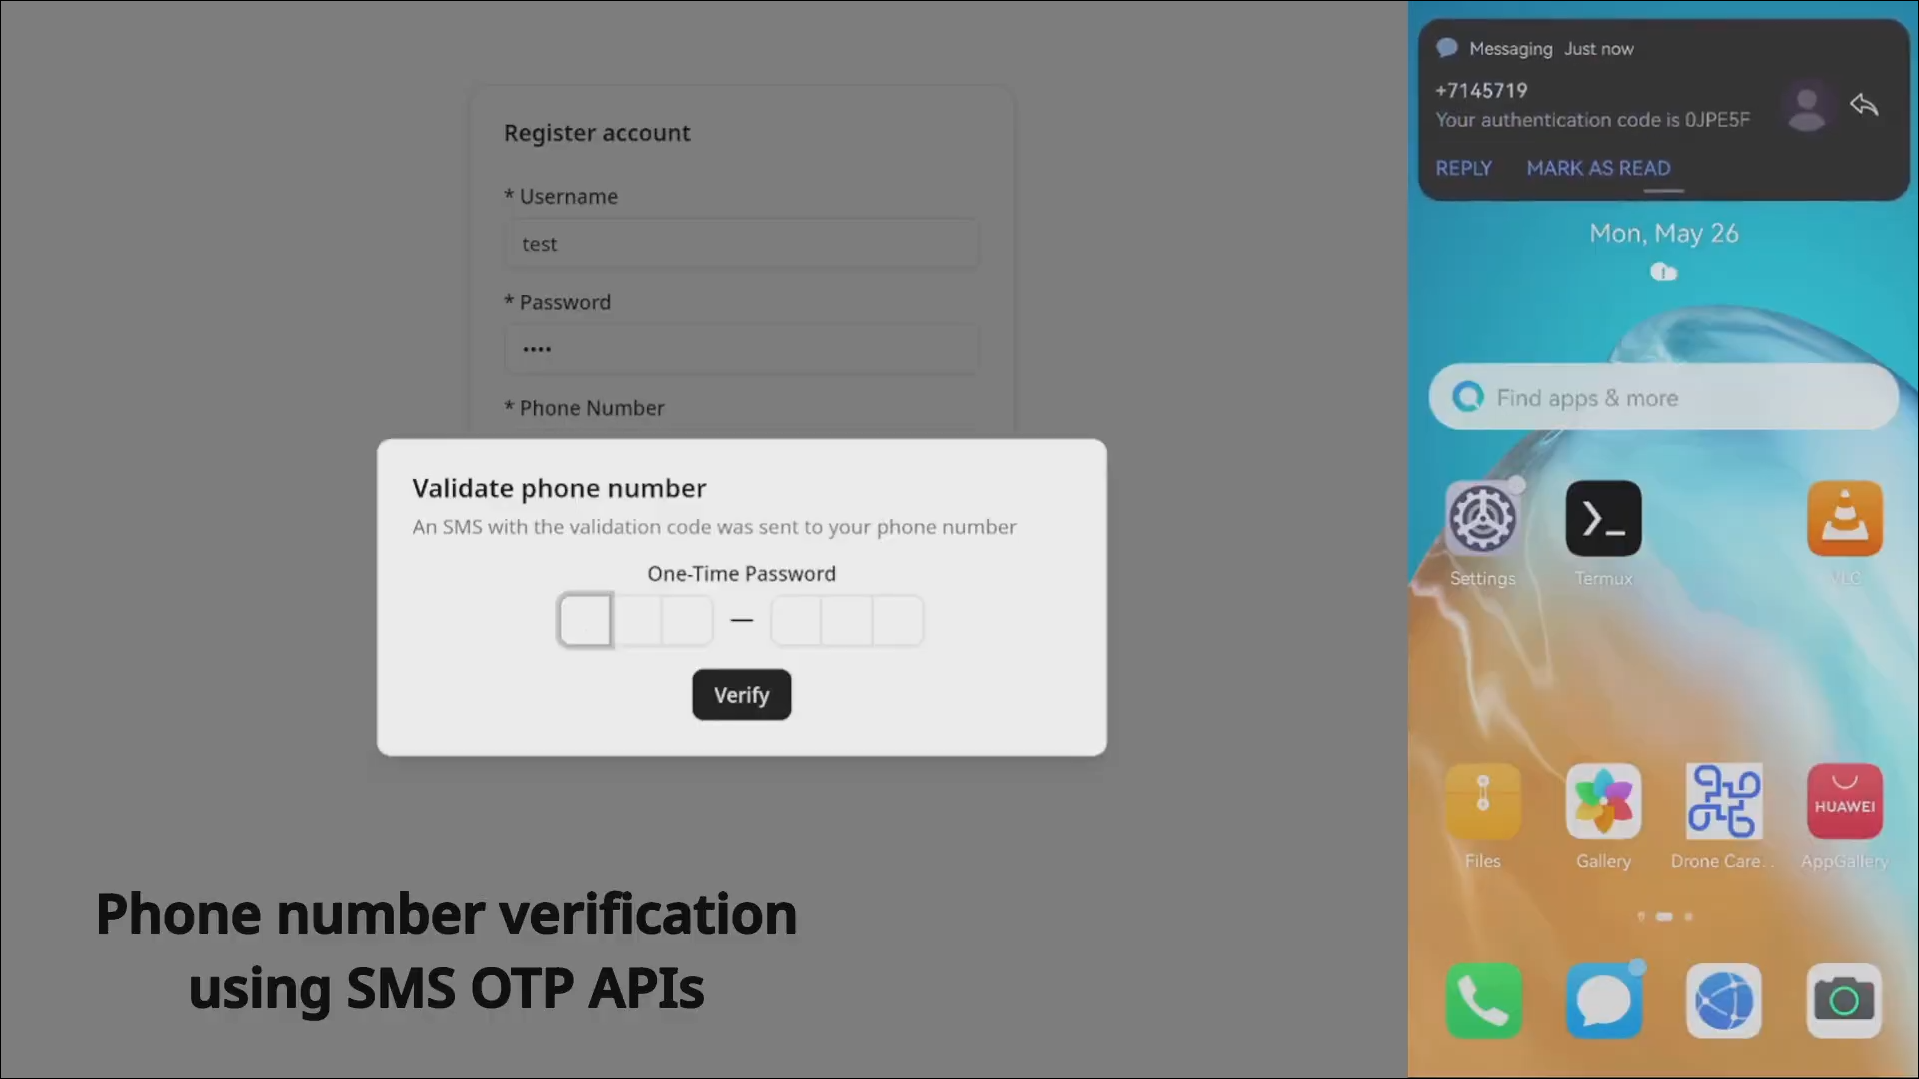
\includegraphics[width=15cm]{figs/SMS_OTP_demo.png}
	}
	\caption{SMS OTP Usage}
	\label{fig:otp}
\end{figure}

\begin{figure}[H]
	\centerline{
		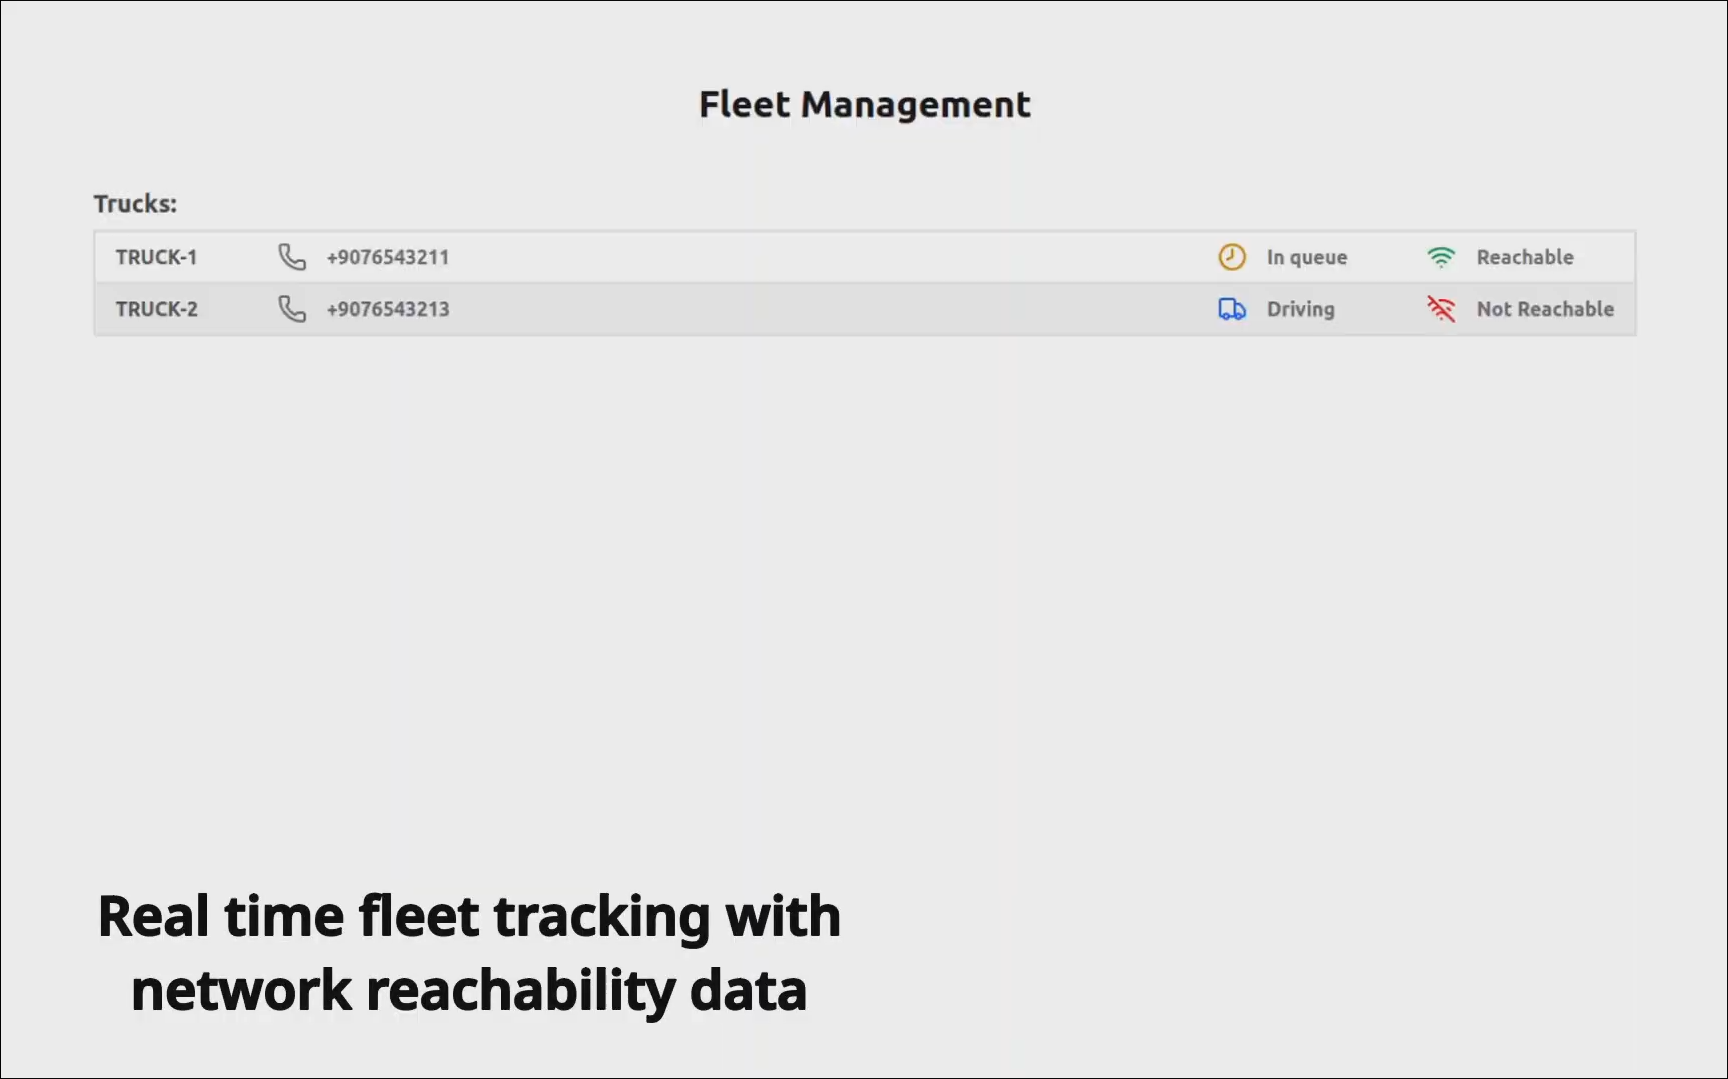
\includegraphics[width=15cm]{figs/reach_demo.png}
	}
	\caption{Device Reachability Status Subscription API Usage}
	\label{fig:reachability}
\end{figure}

\begin{figure}[H]
	\centerline{
		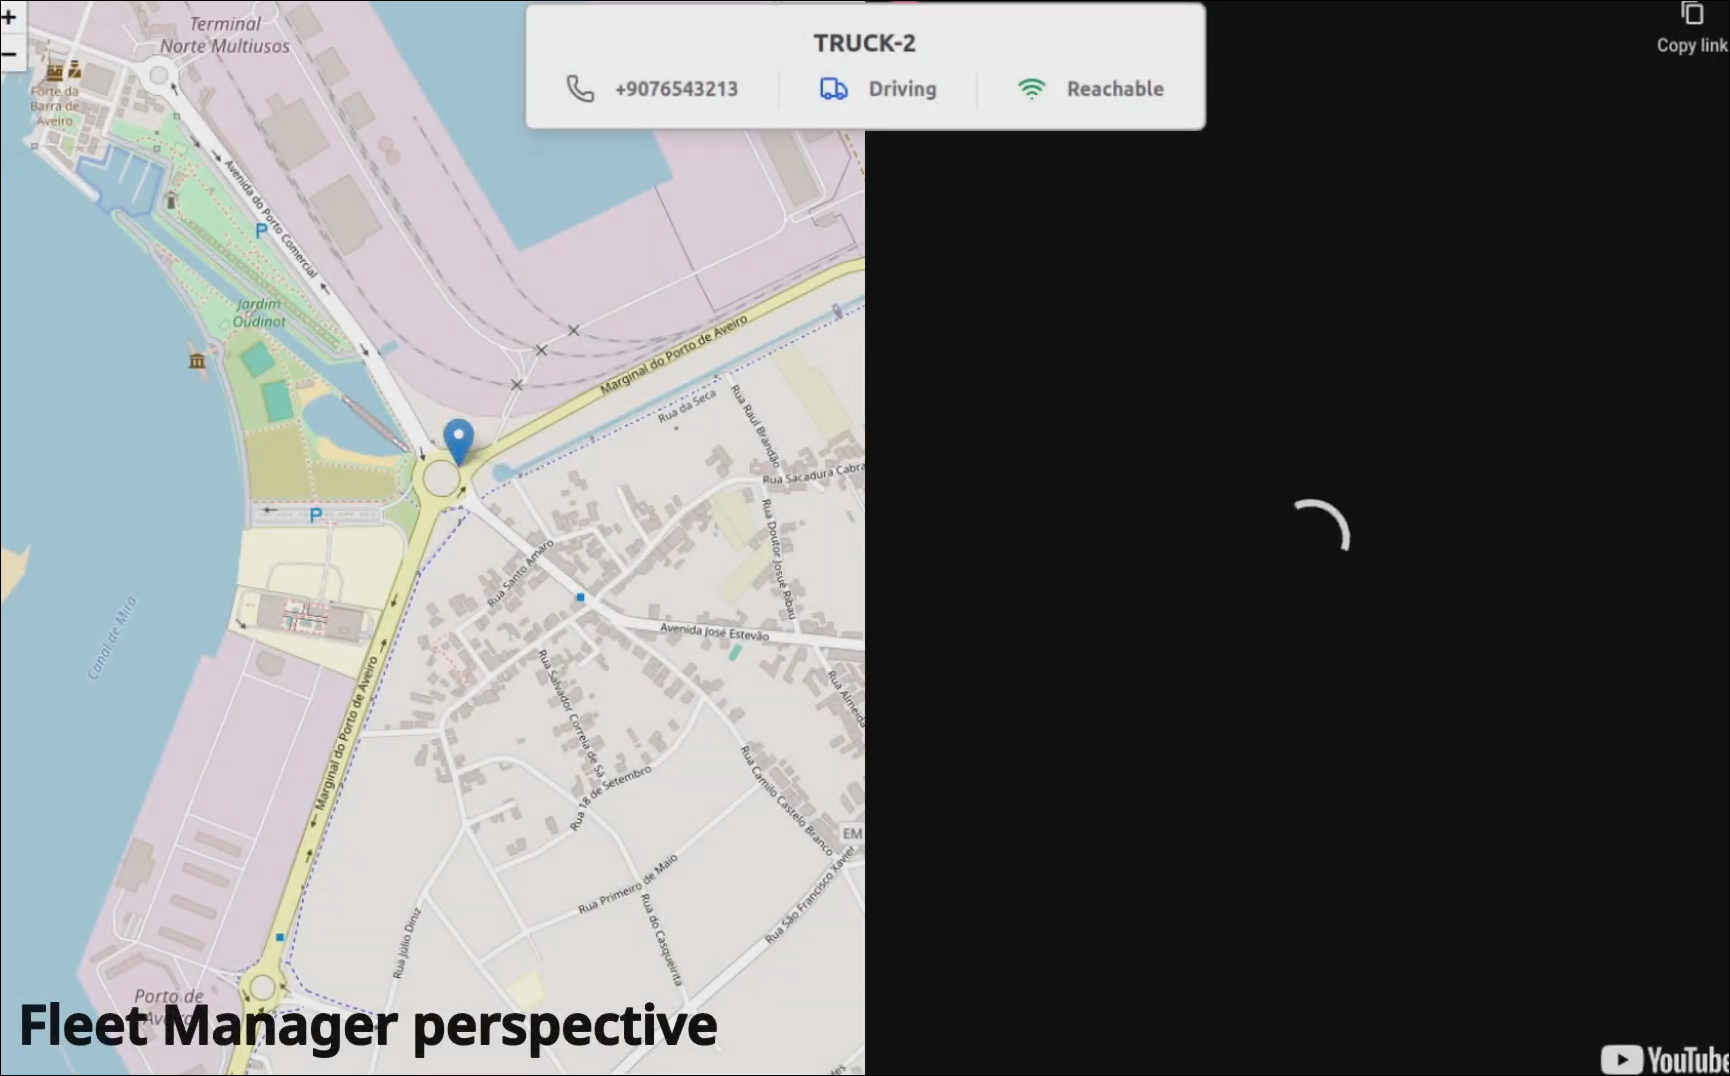
\includegraphics[width=15cm]{figs/Location_demo.png}
	}
	\caption{Location Retrieval API Usage}
	\label{fig:location}
\end{figure}

\begin{figure}[H]
	\centerline{
		\includegraphics[width=15cm]{figs/Geofencing_demo.png}
	}
	\caption{Geofencing Subscription API Usage}
	\label{fig:geofencing}
\end{figure}

\begin{figure}[H]
	\centerline{
		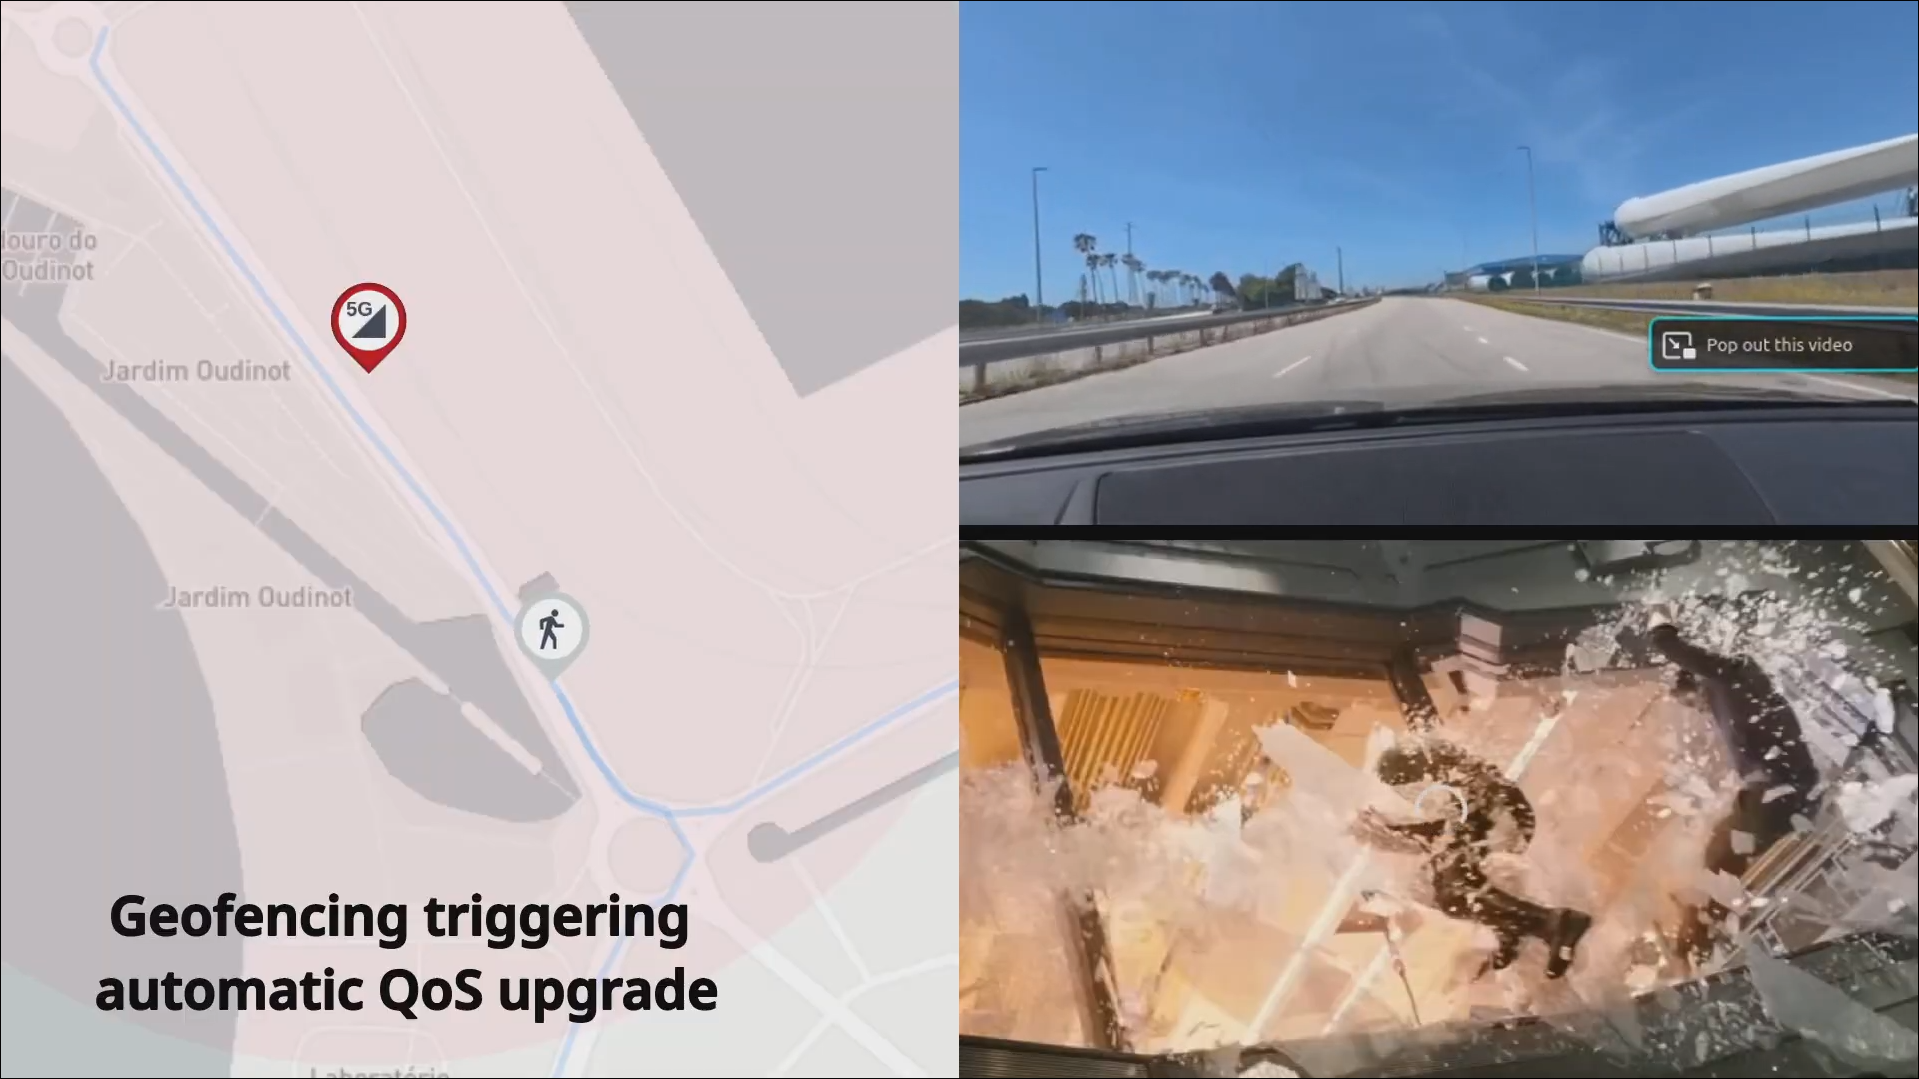
\includegraphics[width=15cm]{figs/QoD_demo.png}
	}
	\caption{Quality on Demand Provisioning API Usage}
	\label{fig:qod}
\end{figure}
